\documentclass[a4paper,12pt]{article} % The document class with options

\usepackage[margin=1in]{geometry}
\usepackage{newtxtext,newtxmath}
\usepackage[T1]{fontenc}
\usepackage{amsmath}
\usepackage{amsfonts}
\usepackage{microtype}
\usepackage{graphicx}
\usepackage{rotating}
% chktex-file 3
% chktex-file 18
% chktex-file 36
% chktex-file 44

\begin{document}
\setlength{\parskip}{1em} 
\setlength{\parindent}{0pt}
\newcommand{\vect}[1]{\mathbf{#1}}

\title{CHBE 552 Problem Set 5}
\author{Jincong Li \\ 60539939}
\date{\today}
\maketitle
\section*{GNM Q1}
\begin{align*}
    \vect{k} &= [kH, kD, k2, KA_{rel}, KC_{rel}]^T \\
    \vect{x} &= [pA]\\
    \vect{f} &= r_1 = kH * KA_{rel} * CA / (KA_{rel} * CA +  CB +  KC_{rel}*CC) \\
    &r_{-1} = kD * CB / (KA_{rel} * CA +  CB +  KC_{rel}*CC)\\
    &r_2 = k2 * CB / (KA_{rel} * CA +  CB +  KC_{rel}*CC)\\
    dCA_{dt} &= -r_1 + r_{-1} \\
    dCB_{dt} &= r_1 - r_{-1} - r_2\\
    dCC_{dt} &= r_2  \\
    \vect{y} &= [CA, CB, CC]\\
\end{align*} 

The sensitivity matrix is computed and embeded in the code. Thus, it could not be presented here explicitly, but I shall provide
the computation procedure here:

For a parameter vector $\boldsymbol{\theta}$ of length $n$, and $m$ residuals, the Jacobian matrix $\mathbf{J}$ is an $m \times n$ matrix. The approximation of the $j$-th column of $\mathbf{J}$ (the derivative of the residuals with respect to the $j$-th parameter) can be calculated as follows:

\begin{enumerate}
    \item \textbf{Slightly Perturb the $j$-th Parameter}: For a small value $\varepsilon$, create a new parameter vector $\boldsymbol{\theta}_\varepsilon$ where only the $j$-th parameter is increased by $\varepsilon$, i.e., 
    \[ \theta_{\varepsilon,j} = \theta_j + \varepsilon. \]
    
    \item \textbf{Calculate the Difference in Predictions}: Use the model function to calculate predictions using $\boldsymbol{\theta}$ and $\boldsymbol{\theta}_\varepsilon$, and compute the difference in the resulting predictions. This difference approximates the change in the residuals caused by the perturbation in the $j$-th parameter.
    
    \item \textbf{Divide by $\varepsilon$}: The approximation of the derivative is the difference in the residuals divided by $\varepsilon$.
\end{enumerate}


From now on, result tables for each model and equestions are presented. In table 1, the final results for
those parameters with their corresponding 95\% confidence intervals in each case are listed.

\begin{table}[ht]
    \centering
    \begin{tabular}{|c|c|c|c|c|c|c|}
    \hline
Iter. & OV & kH & kD& k2& KArel& KCrel \\ \hline
0 & 0.2617 & 0.0281& 0.0063& 0.0038& 1.8969& 1.8059 \\ \hline
1 & 0.0695 & 0.0256& 0.0060& 0.0071& 1.8965& 1.8066\\ \hline
2 & 0.0292 & 0.0242& 0.0056& 0.0091& 1.9006& 1.8053 \\ \hline
3 & 0.0201 & 0.0235& 0.0053& 0.0102& 1.9007& 1.8035  \\ \hline 
4 & 0.0179 & 0.0232& 0.0051& 0.0107& 1.9001& 1.8017 \\ \hline
CI & &(0.020, 0.026)&(0.001, 0.009)&(0.007, 0.014)& (0.840, 2.960)& (0.993, 2.610)\\ \hline
\end{tabular}
\caption{Iteration Details of the Gauss-Newton Marquardt Optimization for Q1}
\label{tab:iteration_details}
\end{table}
Note that the "OV" refers to Objective Function value and CI is confidence level. 

The final values of those parameters are the values in the "iteration \#4" line in table 1. By applying those estimated parameters, figure 1 shows
a comparison between the experimental data in the reference and the estimated data. One can conclude that the values of parameters converge to the reference values
pretty quickly (only five iterations) in the GNM method, though the uncertainty (CI) is larger than the reported values. Thus, the GNM method is really good at with dealing ODE systems 
for parameter estimation. The reason might be the model is relatively simple and the partial derivatives are easy to calculate. Similar results were observed in the second question although the
uncertainties are much larger (details are provided in the next section). The reason could be the implemented GNM code is not robust enough so that when dealing with parameters in different orders of magnitude, the computation is not accurate. 
\begin{figure}[ht]
    \centering
    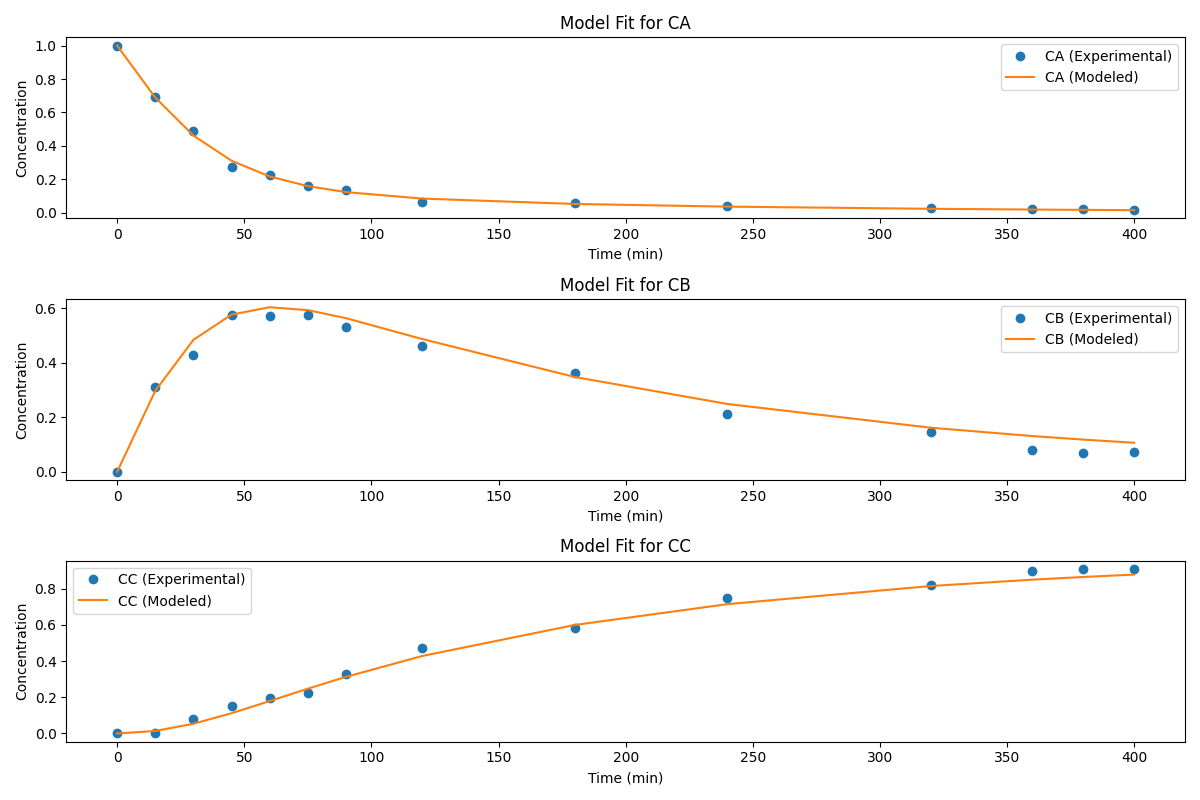
\includegraphics[width=1\textwidth]{Q1_GNM_comp.png}
    \caption{Comparison of Experimental Data with Estimated Data for Q1}
\end{figure}

\clearpage
\section*{GNM Q2}
\begin{align*}
    \vect{k} &= [k1 ,k2, k3, KB_{rel}, KC_{rel}, KD_{rel}]^T \\
    \vect{x} &= [pA]\\
    \vect{f} &= dom = CA + KB_{rel}*CB + KC_{rel}*CC + KD_{rel}*CD\\
    &r_1 = k1*CA/dom\\
    &r_2 = k2*KB_{rel}*CB/dom\\
    &r_3 = k3*KC_{rel}*CC/dom\\
    &dCA_{dt} = -r_1 \\
    &dCB_{dt} = r_1-r_2\\
    &dCC_{dt} = r_2-r_3\\
    &dCD_{dt} = r_3\\
    \vect{y} &= [CA, CB, CC, CD]\\
\end{align*} 

\begin{sidewaystable}
    \centering
    \begin{tabular}{|c|c|c|c|c|c|c|c|}
    \hline
    Iter. & OV & k1 & k2 & k3 & KBrel & KCrel & KDrel\\ \hline
    0 & 2.6549 & 1.4554& 0.4526& 0.6692& 28.0013& 1.8724& 2.8342 \\ \hline
    1 & 1.4312 & 1.4500& 0.0809& 0.5331& 28.0010& 1.8391& 2.8604 \\ \hline
    2 & 0.5558 & 1.4454& 0.0649& 0.2287& 28.0007& 1.8046& 2.8874 \\ \hline
    3 & 0.1784 & 1.4435& 0.0656& 0.1246& 28.0006& 1.7995& 2.8930 \\ \hline
    4 & 0.0542 & 1.4413& 0.0481& 0.0998& 28.0002& 1.7996& 2.8974 \\ \hline
    5 & 0.0153 & 1.4404& 0.0373& 0.0938& 28.0000& 1.7999& 2.8994 \\ \hline 
    6 & 0.0043 & 1.4401& 0.0323& 0.0913& 28.0000& 1.8000& 2.8999 \\ \hline 
    CI& &(1.09, 01.92)& (0.008, 0.072)&(0.012, 0.195)&(17.18, 37.74)& (1.350, 2.386)&(1.819, 3.877)\\ \hline 
    \end{tabular}
    \caption{Iteration Details of the Gauss-Newton Marquardt Optimization for Q2}
    \label{tab:iteration_details}
    \end{sidewaystable}
The final values of those parameters are the values in the "iteration \#6" line in table 2. And by 
applying those estimated parameters, figure 2 shows
a comparision between the experimental data in the reference and the estimated data.
\clearpage

\begin{figure}[ht]
    \centering
    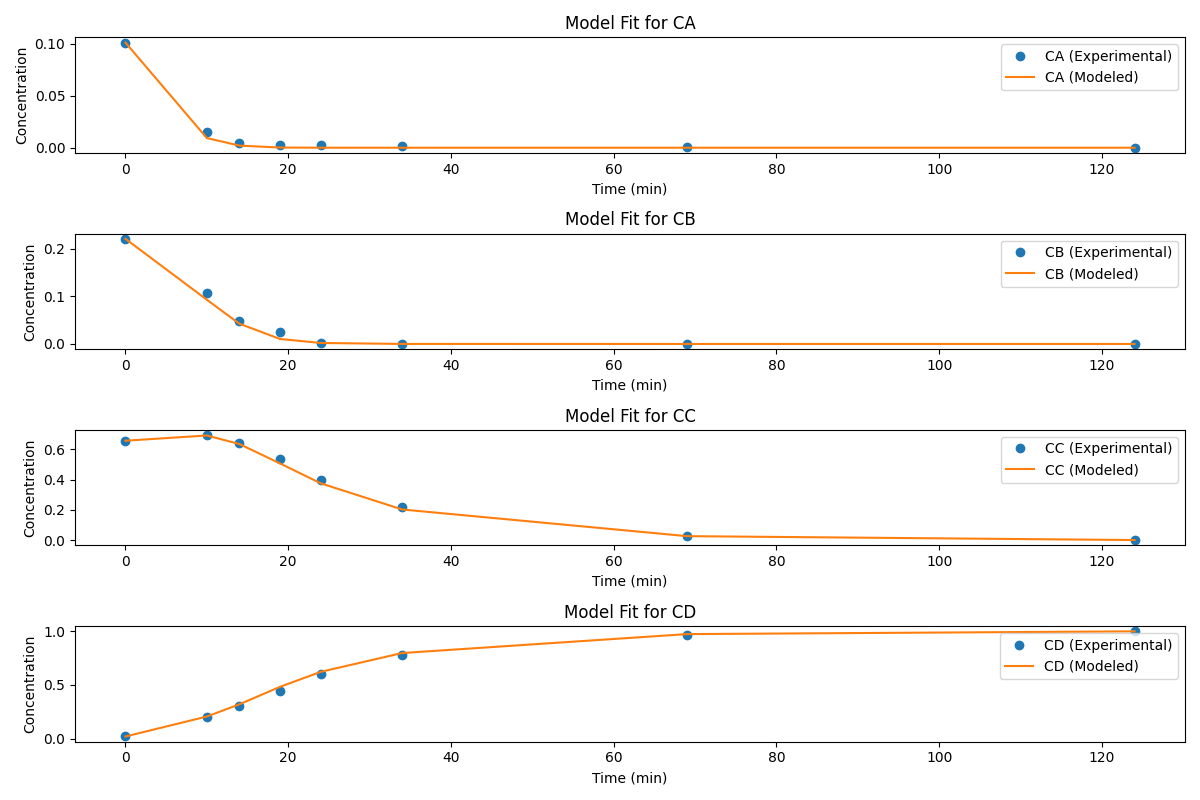
\includegraphics[width=1\textwidth]{Q2_GNM_comp.png}
    \caption{Comparison of Experimental Data with Estimated Data for Q2}
\end{figure}
\clearpage
\section*{LJ}
In table 3, the results of those parameters estimated by the Luus-Jaakola Method are presented. As we can see, some of them do not agree with
the reference values. whereas the some parameters are close to the reference values, such as the KArel and KBrel in Q1. As stated in the last assignment, the Luus-Jaakola Method is naturelly a random process of seeking global 
minimum, the result highly relies on the initial condition/guess of the parameters as well as the general shape with respective to each parameters,
which means there could be multiple local/global minimum. 
Given in limited performance/executing time of the code, in this case, the Luus-Jaakola Method did not reach the real 
solution that we are looking for again. By the experience with tuning parameters in the third assignment, one could definitely
make the LJ method converge to the real solution but it requires too much effort and the time limitation does not allow it. 
Thus, with further work, the LJ method could also return useful information.
\begin{table}[ht]
    \caption{LJ Method Results}
    \centering
    \begin{tabular}{|c|c|c|c|c|c|c|}
        \hline
        Q1 &  kH & kD& k2& KArel& KCrel & \\
        \hline   
        &  0.4921&  0.0055&  0.0001&  1.9468&  1.7930&  \\
        \hline
        Q2 & k1 & k2 & k3 & KBrel & KCrel & KDrel\\
        \hline
        & 3.0003&0.0835& 0.0026&50.0000& 0.3061& 4.9920 \\
        \hline
    \end{tabular}
\end{table}

\end{document}